\chapter{量子機械学習におけるコスト関数の勾配の分散の下界}\label{chap:lower-bound}
この章では、コスト関数の勾配の分散の下界のスケーリングについて調べる。
\ref{sec:cost1}~節では、入力データがガウス分布に従うという仮定の下、絶対誤差のコスト関数 $\calL_{\mathrm{MAE}}(\bs{\th}) = \frac1N\sum_{i=1}^N \;|\ell_i(\bs{\th}) - y_i|$ の勾配の分散の下界を計算する。
\ref{sec:cost2}~節では、二乗誤差のコスト関数 $\calL_{\mathrm{MSE}}(\bs{\th}) = \frac1N\sum_{i=1}^N \;\qty(\ell_i(\bs{\th}) - y_i)^2$ や交差エントロピー誤差のコスト関数 $\calL_{\mathrm{LOG}}(\bs{\th}) = \frac1N\sum_{i=1}^N \;[-y_i\log\ell_i(\bs{\th}) - (1-y_i)\log(1-\ell_i(\bs{\th}))]$ の勾配の分散を、絶対誤差のコスト関数の勾配の分散から推定する。

\section{絶対誤差のコスト関数の勾配の分散}\label{sec:cost1}
この節では、量子回路の構造は図~\ref{fig:circuit-setting}で与えられるものとする。すなわち、学習回路は $\xi$ 個の $s$ 量子ビットユニタリからなり、全量子ビット数は $n=s\times\xi$ である。
そして、2値分類 $y_i \in \{0,1\}$ の問題設定において、絶対誤差のコスト関数の勾配の分散の下界を計算する。

コスト関数が 
$$
    \calL_{\mathrm{MAE}}(\bs{\th}) = \frac1N\sum_{i=1}^N \,|\ell_i(\bs{\th}) - y_i|,\quad \ell_i(\bs{\th}) = \Tr[\rho_i(\bs{\th})\,O_\rmL],\quad O_\rmL = \frac{1}{n} \sum_{j=1}^{n}\dyad{0}_{j} \otimes \bbid_{\bar{j}}
$$
で与えられるとき、コスト関数の勾配は、 $\pd_\nu := \pd/\pd\th_\nu$, $w_i := \sgn(\ell_i(\bs{\th}) - y_i)$ として、
\begin{align}
    \pd_\nu\calL_{\mathrm{MAE}}(\bs{\th})
    &= \frac1N\sum_{i=1}^N \;w_i \cdot \pd_\nu\ell_i(\bs{\th})
\end{align}
と表せる。
ただし、$\ell_i(\bs{\th}) \in [0,1]$ であることから $w_i$ と $y_i$ は次のように対応する。
\begin{align}
    w_i =
    \begin{cases}
        \;\;\,1 & \text{if}\quad y_i = 0\\
             -1 & \text{if}\quad y_i = 1
    \end{cases}
\end{align}

ここで、学習回路の各 $s$ 量子ビットユニタリがユニタリ $2$--デザインを成すと仮定する。また、証明\ref{proof:qml-upper-var}で示したように、勾配の平均は $0$ である。よって、勾配の分散は次のように計算できる。
\begin{align}
    \Var_{V(\bs{\th})}[\pd_\nu\calL_{\mathrm{MAE}}(\bs{\th})]
    &= \E_{V(\bs{\th})}[(\pd_\nu\calL_{\mathrm{MAE}}(\bs{\th}))^2]\nonumber\\
    &= \frac{1}{N^2}\sum_{i,j=1}^N\;
    w_i\, w_j
    \E_{V(\bs{\th})}[\pd_\nu\ell_i(\bs{\th})\cdot\pd_\nu\ell_j(\bs{\th})]\label{eq:abs-cost-variance}
\end{align}

$\E_{V(\bs{\th})}[\pd_\nu\ell_i(\bs{\th})\cdot\pd_\nu\ell_j(\bs{\th})]$ は、論文~\cite{cerezo2021cost}の結果を拡張することで次のように計算できる。略証は\ref{sec:prf-covariance}~節を参照。
\begin{screen}
    \begin{corollary}\label{cor:covariance}
        (論文~\cite{cerezo2021cost}の Supplementary Note 5, B の拡張された結果)
        量子回路の構造は図~\ref{fig:circuit-setting}で与えられ、学習回路の各 $s$ 量子ビットユニタリがユニタリ $2$--デザインを成すとき、次の等式が成り立つ。
        \begin{align}
            \E_{V(\bs{\th})}\qty[\pd_\nu\ell_i(\bs{\th})\,\cdot\,\pd_\nu\ell_j(\bs{\th})] = r_{n,s}\qty(\Tr\qty[\rho_i^{(h)}\rho_j^{(h)}]-\frac{1}{2^s}),
            \quad r_{n,s} := \frac{s\,2^{3(s-1)}}{n^2(2^{2s}-1)^2}
        \end{align}
    \end{corollary}
\end{screen}

よって、式~\eqref{eq:abs-cost-variance}は次のように書き換えられる。
\begin{align}\label{eq:abs-cost-variance-2}
    \Var_{V(\bs{\th})}[\pd_\nu\calL_{\mathrm{MAE}}(\bs{\th})]
    &= \frac{r_{n,s}}{N^2}
    \sum_{i,j=1}^N\; w_i\, w_j\,
    \qty(\Tr[\rho_i^{(h)}\rho_j^{(h)}]-\frac{1}{2^s})\\
    &=
    \frac{r_{n,s}}{N^2}
    \qty[
        \sum_{w_i=w_j}^N\;
        \qty(\Tr[\rho_i^{(h)}\rho_j^{(h)}]-\frac{1}{2^s})
        -
        \sum_{w_i\neq w_j}^N\;
        \qty(\Tr[\rho_i^{(h)}\rho_j^{(h)}]-\frac{1}{2^s})
    ]
\end{align}

上の表式から、入力状態に依存する $\Tr[\rho_i^{(h)}\rho_j^{(h)}]$ が重要であり、$\Tr[\rho_i^{(h)}\rho_j^{(h)}]$ が同じラベルの場合と異なるラベルの場合でどのようにスケーリングするかが、勾配の分散に影響することがわかる
\footnote{
論文\cite{garcia-martin2023deep}においては、入力状態が十分に分離していることを、同じラベルの入力状態間のカーネルと異なるラベルの入力状態間のカーネルが次のようにスケールことと述べている。
\begin{alignat*}{2}
    \Tr[\rho_i \rho_{i^{\prime}}] &\in \Omega\qty(\frac{1}{\poly(n)}), \quad&\text{if} \quad y_i=y_{i^{\prime}} \\
    \Tr[\rho_i \rho_{i^{\prime}}] &\in \calO\qty(\frac{1}{2^n}), \quad&\text{if} \quad y_i \neq y_{i^{\prime}}
\end{alignat*}
}。

式\eqref{eq:abs-cost-variance-2}をさらに変形すると、次のようになる。
\begin{align}
    \Var_{V(\bs{\th})}[\pd_\nu\calL_{\mathrm{MAE}}(\bs{\th})]
    &=
    r_{n,s}\;
    \qty(\Tr[(\overline{\rho})^2] - \frac{w^2}{2^s}) \label{eq:abs-cost-variance-3}
\end{align}
ただし、$w := \frac1N\sum_{i=1}^N w_i,\; \overline{\rho} := \frac{1}{N}\sum_{i=1}^N w_i\rho_i^{(h)}$ とした。前者は $w_i = \pm1$ であることに注意すると、$\abs{w} \leq 1$ である。
特に、$\#\{y_i|y_i=0\} = \#\{y_i|y_i=1\} = N/2$ ならば $w = 0$ であり、$\#\{y_i|y_i=0\} = N$ または $\#\{y_i|y_i=1\} = N$ ならば $|w| = 1$ である。
後者は、論文\cite{hubregtsen2022training}において述べられているように Kernel Alignment と類似した量である。簡単のため、$\overline{\rho}$ と表しているが、この量自体は密度演算子とは限らないことに注意する。なぜなら、$\Tr[\overline{\rho}] = w$ だからである。
% また、平均した状態の純粋度 $\Tr[(\bar{\rho})^2]$ はカーネル $\kappa_{FQ}(\bs{x},\bs{y})$ の平均として解釈することができることに言及しておく。
% \footnote{
%     次の変形を行うことができる。
%     \begin{align}
%         \Tr[(\bar{\rho})^2]
%         = \Tr\qty[\qty(\int \rho(\bs{x}_i)\,\mu(d\bs{x}))^2]
%         = \iint\Tr[\rho(\bs{x})\rho(\bs{y})]\mu(d\bs{x})\mu(d\bs{y})
%         =:\iint\kappa_{FQ}(\bs{x},\bs{y})\;\mu(d\bs{x})\mu(d\bs{y})
%     \end{align}
% }


さらに、$\overline{\rho}_\pm := \frac{1}{N}\sum\limits_{i,(w_i=\pm1)} \rho_i^{(h)}$ として、$\overline{\rho}$ を変形すると次のようになる。
\begin{align}
    \Tr[(\overline{\rho})^2]
    =  \Tr[(\overline{\rho}_+ - \overline{\rho}_-)^2]
    = D_{HS}(\overline{\rho}_+,\, \overline{\rho}_-)
\end{align}
したがって、それぞれのラベルの平均入力状態である $\overline{\rho}_+$ と $\overline{\rho}_-$ の差が大きいほど、下界も大きくなることがわかる。



\subsection{下界のスケーリング(1)}\label{sec:lower-bound-1}
ここでは、先行研究~\cite{li2022concentration}で得られた結果を拡張し、コスト関数の勾配の分散の下界を計算する。
入力データの各成分はガウス分布に従い、入力回路は図~\ref{fig:circuit-concentration-1}のように $R_y$ ゲートのみで構成されているとする。
このとき、次の定理が成り立つ。証明は\ref{sec:prf-concentration-1}~節を参照。

\begin{screen}
    \begin{theorem}\label{thm:concentration-1}
        (論文~\cite{li2022concentration}の Theorem 1 の拡張された結果)
        $\calX = \{\bs{x}\}$, $\calZ = \{\bs{z}\}$ はそれぞれラベル $y_i=0$ と $y_i=1$ に属する入力データセットであり、$|\calX|:|\calZ| = p:q\;(p+q=1)$ であるとする。
        そして、各データサンプルを次のように表記する:$\bs{x} = (\bs{x}_{j})_{j=1}^n,\, \bs{x}_{j} = (x_{j,d})_{d=1}^L$, $\bs{z} = (\bs{z}_{j})_{j=1}^n,\, \bs{z}_{j} = (z_{j,d})_{d=1}^L$。異なるラベルに属する入力データを量子回路に同時には入力しないとする。
        入力データの各成分の分布は $x_{j,d} \sim \calN(\mu_{x|j,d}, \sigma_{x|j,d}^2)$, $z_{j,d} \sim \calN(\mu_{z|j,d}, \sigma_{z|j,d}^2)$ であり、分散は $\sigma_{\min} \leq \sigma_{x|\fa j,d},\, \sigma_{z|\fa j,d} \leq \sigma_{\max}$ を満たすとする。また、量子回路は図~\ref{fig:circuit-concentration-1}のように構成されている。ただし、$1\leq j\leq n,\, 1\leq d\leq L$ である。
        このとき、$\bar{\rho} = p\E_\calX[\rho^{(h)}(\bs{x})] - q\E_\calZ[\rho^{(h)}(\bs{z})]$ について次の不等式が成り立つ。
        \begin{align}
            \frac{1}{2^s}
            \qty[w^2 + \sum_{j=1}^s \qty(p\,e^{-\Sigma_{x|j}/2} - q\,e^{-\Sigma_{z|j}/2})^2]
            \leq \Tr[(\bar{\rho})^2]
            \leq \frac{1}{2^s} (1 + e^{-L\,\sigma_{\min}^2})^s
        \end{align}
        ただし、$n,s$ は量子ビット数($n=s\times\xi$)、$L$ は入力回路の層数、$w = p - q$, $\Sigma_{x|j}:=\sum_{d=1}^L \sigma_{x|j,d}^2$, $\Sigma_{z|j}:=\sum_{d=1}^L \sigma_{z|j,d}^2$ である。
    \end{theorem}
\end{screen}
この定理においては、$\th_\nu$ が含まれる $h\,(1\leq h\leq\xi)$ 番目の $s$ 量子ビットについてだけ考えればよいことに注意する。


\newcommand{\bgate}[1]{\gate[wires=1,style={fill=cyan!50}]{#1}}
\newcommand{\rgate}[1]{\gate[wires=4,style={fill=red!30}]{#1}}
\begin{figure}[H]
    \centering
    \begin{tikzpicture}
    \node[scale=0.9]{
        \begin{quantikz}
            \lstick{$\ket{0}$} & \bgate{R_y(x_{1,1})}    & \bgate{R_y(x_{1,2})}    &\ \ldots\ & \bgate{R_y(x_{1,L-1})}    & \bgate{R_y(x_{1,L})}    &\rgate{V_1(\bs{\th}_1)}& \meter{} \\
            \lstick{$\ket{0}$} & \bgate{R_y(x_{2,1})}    & \bgate{R_y(x_{2,2})}    &\ \ldots\ & \bgate{R_y(x_{2,L-1})}    & \bgate{R_y(x_{2,L})}    & \qw                     & \meter{} \\
            \wave&&&&&&&&&\\
            \lstick{$\ket{0}$} & \bgate{R_y(x_{s,1})}    & \bgate{R_y(x_{s,2})}    &\ \ldots\ & \bgate{R_y(x_{s,L-1})}    & \bgate{R_y(x_{s,L})}    & \qw                     & \meter{}\\
            \lstick{$\ket{0}$} & \bgate{R_y(x_{s+1,1})}  & \bgate{R_y(x_{s+1,2})}  &\ \ldots\ & \bgate{R_y(x_{s+1,L-1})}  & \bgate{R_y(x_{s+1,L})}  &\rgate{V_2(\bs{\th}_2)}& \meter{} \\
            \lstick{$\ket{0}$} & \bgate{R_y(x_{s+2,1})}  & \bgate{R_y(x_{s+2,2})}  &\ \ldots\ & \bgate{R_y(x_{s+2,L-1})}  & \bgate{R_y(x_{s+2,L})}  & \qw                     & \meter{} \\
            \wave&&&&&&&&&\\
            \lstick{$\ket{0}$} & \bgate{R_y(x_{2s,1})}   & \bgate{R_y(x_{2s,2})}   &\ \ldots\ & \bgate{R_y(x_{2s,L-1})}   & \bgate{R_y(x_{2s,L})}   & \qw                     & \meter{}\\
            \wave&&&&&&&&&\\
            \lstick{$\ket{0}$} & \bgate{R_y(x_{n-s+1,1})}& \bgate{R_y(x_{n-s+1,2})}&\ \ldots\ & \bgate{R_y(x_{n-s+1,L-1})}& \bgate{R_y(x_{n-s+1,L})}&\rgate{V_\xi(\bs{\th}_\xi)}& \meter{} \\
            \lstick{$\ket{0}$} & \bgate{R_y(x_{n-s+2,1})}& \bgate{R_y(x_{n-s+2,2})}&\ \ldots\ & \bgate{R_y(x_{n-s+2,L-1})}& \bgate{R_y(x_{n-s+2,L})}& \qw                     & \meter{} \\
            \wave&&&&&&&&&\\
            \lstick{$\ket{0}$} & \bgate{R_y(x_{n,1})}    & \bgate{R_y(x_{n,2})}    &\ \ldots\ & \bgate{R_y(x_{n,L-1})}    & \bgate{R_y(x_{n,L})}    & \qw                     & \meter{}
        \end{quantikz}};
    \end{tikzpicture}
    \caption{$n = s\times\xi$ 量子ビットからなる量子回路。入力回路は $L$ 層の $R_y$ ゲートからなる。学習回路は $\xi$ 個の $s$ 量子ビットユニタリからなる。}
    \label{fig:circuit-concentration-1}
\end{figure}


定理~\ref{thm:concentration-1}と式~\eqref{eq:abs-cost-variance-3}より、直ちに次の定理が導かれる。
\begin{screen}
    \begin{theorem}\label{thm:lower-bound-1}
        系\ref{cor:covariance}と定理\ref{thm:concentration-1}の条件のもとで、
        絶対誤差のコスト関数の勾配の分散は上下から次のように抑えられる。
        \begin{align}
            \frac{r_{n,s}}{2^s}\;
            \sum_{j=1}^s \qty(p\,e^{-\Sigma_{x|j}/2} - q\,e^{-\Sigma_{z|j}/2})^2
            \leq \Var_{V(\bs{\th})}[\pd_\nu\calL_{\mathrm{MAE}}(\bs{\th})]
            \leq \frac{r_{n,s}}{2^s}\;\qty[\qty(1 + e^{-L\,\sigma_{\min}^2})^s - w^2]
        \end{align}
        ただし、$r_{n,s} := \frac{s\,2^{3(s-1)}}{n^2(2^{2s}-1)^2}$, $w = p - q$ である。
    \end{theorem}
\end{screen}

\subsubsection{$|\calX|:|\calZ| = 1:1$ の場合}
$|\calX|:|\calZ| = 1:1 \iff p = q = 1/2,\, w = 0$ の場合、定理\ref{thm:lower-bound-1}は次のようになる。
\begin{align}
    \frac{r_{n,s}}{2^{s+2}}\;
    \sum_{j=1}^s
    \qty(e^{-\Sigma_{x|j}/2}- e^{-\Sigma_{z|j}/2})^2
    \leq \Var_{V(\bs{\th})}[\pd_\nu\calL_{\mathrm{MAE}}(\bs{\th})]
    \leq r_{n,s}\;\qty(\frac{1 + e^{-L\,\sigma_{\min}^2}}{2^s})^s
    \leq r_{n,s}
\end{align}

これより $e^{-\Sigma_{x|j}/2},\,e^{-\Sigma_{z|j}/2}$ の差が大きいほど、下界が大きくなることがわかる。しかし、$(e^{-\Sigma_{x|j}/2}- e^{-\Sigma_{z|j}/2})^2$ は層数 $L$ を増やすと指数関数的に小さくなる。
また、すべての $j$ について $e^{-\Sigma_{x|j}/2} = e^{-\Sigma_{z|j}/2}$ である場合、下界は $0$ となり意味をなさない\footnote{極端な例として、$\calX = \calZ$ の場合は、$\calL_{\mathrm{MAE}}(\bs{\th}) = 1/2$ となるため、勾配は $0$、したがって勾配の分散も $0$ となる。ゆえに、下界が $0$ となることもあり得る。}。

一方で、$s \in \order{\poly(n)}$ ならば、上界は指数関数的に減少するため、バレンプラトーとなることがわかる。

\subsubsection{$|\calX|:|\calZ| = 1:0$ の場合}
異常検知などに用いられる One class classification~\cite{khan2014oneclass}の場合は、$|\calX|:|\calZ| = 1:0 \iff p = 1,\, q = 0,\, w = 1$ となる。このとき、定理\ref{thm:lower-bound-1}は次のようになる。
\begin{align*}
    &\frac{r_{n,s}}{2^s}\;
    \sum_{j=1}^s e^{-\Sigma_{x|j}}
    \leq \Var_{V(\bs{\th})}[\pd_\nu\calL_{\mathrm{MAE}}(\bs{\th})]
    \leq \frac{r_{n,s}}{2^s}\;\qty[\qty(1 + e^{-L\,\sigma_{\min}^2})^s - 1]
\end{align*}

$\Sigma_{x|j} \leq L\,\sigma_{\max}^2$ であるから、$se^{-L\,\sigma_{\max}^2} \leq \sum_{j=1}^s e^{-\Sigma_{x|j}}$ が成り立つ。
これと、$[(1 + e^{-L\,\sigma_{\min}^2})^s - 1]/2^s \leq 1$ であることから、定理\ref{thm:lower-bound-1}は次のようになる。
\begin{align}
    &\frac{r_{n,s} s}{2^s}\;e^{-L\,\sigma_{\max}^2}
    \leq \Var_{V(\bs{\th})}[\pd_\nu\calL_{\mathrm{MAE}}(\bs{\th})]
    \leq r_{n,s}
\end{align}

$s$ と $\sigma_{\max}^2$ が固定されているとすると、勾配の分散の下界が量子ビット数 $n$ に関して $\order{1/\poly(n)}$ でスケールするためには、$L \in \order{\log{n}}$ でなければならない。
ところで、\ref{sec:quantum-kernel}節の量子カーネル法の説明で述べた Bandwidth というハイパーパラメーターを導入すれば、入力するデータの分散を調整することができる。よって分散の最大値が $\sigma_{\max}^2 \in \order{\log{n}}/L$ を満たすように Bandwidth を調整すれば、$L\,\sigma_{\max}^2 \in \order{\log{n}}$ となるようにできる。しかし、この手法によってバレンプラトーが回避できても、汎化性能に悪影響を及ぼす可能性があることに注意する。

一方、上界については $s \in \order{\poly(n)}$ のとき、上界は指数関数的に減少するため、バレンプラトーとなることがわかる。


\subsection{下界のスケーリング(2)}
ここでも先程と同様に、先行研究~\cite{li2022concentration}で得られた結果を拡張し、コスト関数の勾配の分散の下界を計算する。
ただし、この節では $p = 1,\, q = 0$ である場合のみを考える。
入力データの各成分はガウス分布に従い、入力回路は図~\ref{fig:circuit-concentration-2}のように構成されているとする。
このとき、次の定理が成り立つ。略証は\ref{sec:prf-concentration-2}~節を参照。
\begin{screen}
    \begin{theorem}\label{thm:concentration-2}
        (論文~\cite{li2022concentration}の Theorem 2 の拡張された結果)
        $\calX = \{\bs{x}\}$ はラベル $y_i=0$ に属する入力データセットであるとする。
        そして、各データサンプルを次のように表記する:$\bs{x} = (\bs{x}_{j})_{j=1}^n,\, \bs{x}_{j} = (\bs{x}_{j,d})_{d=1}^L,\,\bs{x}_{j,d} = (x_{j,d,1},x_{j,d,2},x_{j,d,3})$。
        入力データの各成分の分布は $x_{j,d,k} \sim \calN(\mu_{x|j,d,k}, \sigma_{x|j,d,k}^2)$ であり、分散は $\sigma_{\min} \leq \sigma_{x|\fa j,d,k} \leq \sigma_{\max}$ を満たすとする。また、量子回路は図~\ref{fig:circuit-concentration-2}のように構成されている。ただし、$1\leq j\leq n,\, 1\leq d\leq L,\,1\leq k\leq 3$ である。
        このとき、$\bar{\rho} := \E_\calX[\rho^{(h)}(\bs{x})]$ について次の不等式が成り立つ。
        \begin{align}
            \frac{1}{2^s} + e^{-3s\,L\,\sigma_{\max}^2}
            \leq \Tr[(\bar{\rho})^2]
            \leq \frac{1}{2^s} + e^{-L\,\sigma_{\min}^2}
        \end{align}
        ただし、$n,s$ は量子ビット数($n=s\times\xi$)、$L$ は入力回路の層数である。
    \end{theorem}
\end{screen}
この定理においては、$\th_\nu$ が含まれる $h\,(1\leq h\leq\xi)$ 番目の $s$ 量子ビットについてだけ考えればよいことに注意する。


\newcommand{\bbgate}[1]{\gate[wires=4,style={fill=cyan!50}]{#1}}
\begin{figure}
    \centering
    \begin{tikzpicture}
    \node[scale=0.7]{
        \begin{quantikz}
            \lstick{$\ket{0}$} & \bgate{U_3(\bs{x}_{1,1})}    &\bbgate{Etg_{1,1}}& \bgate{U_3(\bs{x}_{1,2})}    &\bbgate{Etg_{1,2}}&\ \ldots\ & \bgate{U_3(\bs{x}_{1,L-1})}    &\bbgate{Etg_{1,L-1}}& \bgate{U_3(\bs{x}_{1,L})}    &\rgate{V_1(\bs{\th}_1)}& \meter{} \\
            \lstick{$\ket{0}$} & \bgate{U_3(\bs{x}_{2,1})}    & \qw           & \bgate{U_3(\bs{x}_{2,2})}    & \qw           &\ \ldots\ & \bgate{U_3(\bs{x}_{2,L-1})}    & \qw               & \bgate{U_3(\bs{x}_{2,L})}    & \qw                     & \meter{} \\
            \wave&&&&&&&&&&\\
            \lstick{$\ket{0}$} & \bgate{U_3(\bs{x}_{s,1})}    & \qw           & \bgate{U_3(\bs{x}_{s,2})}    & \qw           &\ \ldots\ & \bgate{U_3(\bs{x}_{s,L-1})}    & \qw               & \bgate{U_3(\bs{x}_{s,L})}    & \qw                     & \meter{}\\
            \lstick{$\ket{0}$} & \bgate{U_3(\bs{x}_{s+1,1})}  &\bbgate{Etg_{2,1}}& \bgate{U_3(\bs{x}_{s+1,2})}  &\bbgate{Etg_{2,2}}&\ \ldots\ & \bgate{U_3(\bs{x}_{s+1,L-1})}  &\bbgate{Etg_{2.L-1}}& \bgate{U_3(\bs{x}_{s+1,L})}  &\rgate{V_2(\bs{\th}_2)}& \meter{} \\
            \lstick{$\ket{0}$} & \bgate{U_3(\bs{x}_{s+2,1})}  & \qw           & \bgate{U_3(\bs{x}_{s+2,2})}  & \qw           &\ \ldots\ & \bgate{U_3(\bs{x}_{s+2,L-1})}  & \qw               & \bgate{U_3(\bs{x}_{s+2,L})}  & \qw                     & \meter{} \\
            \wave&&&&&&&&&&\\
            \lstick{$\ket{0}$} & \bgate{U_3(\bs{x}_{2s,1})}   & \qw           & \bgate{U_3(\bs{x}_{2s,2})}   & \qw           &\ \ldots\ & \bgate{U_3(\bs{x}_{2s,L-1})}   & \qw               & \bgate{U_3(\bs{x}_{2s,L})}   & \qw                     & \meter{}\\
            \wave&&&&&&&&&&\\
            \lstick{$\ket{0}$} & \bgate{U_3(\bs{x}_{n-s+1,1})}&\bbgate{Etg_{\xi,1}}& \bgate{U_3(\bs{x}_{n-s+1,2})}&\bbgate{Etg_{\xi,2}}&\ \ldots\ & \bgate{U_3(\bs{x}_{n-s+1,L-1})}&\bbgate{Etg_{\xi,L-1}}& \bgate{U_3(\bs{x}_{n-s+1,L})}&\rgate{V_\xi(\bs{\th}_\xi)}& \meter{} \\
            \lstick{$\ket{0}$} & \bgate{U_3(\bs{x}_{n-s+2,1})}& \qw           & \bgate{U_3(\bs{x}_{n-s+2,2})}& \qw           &\ \ldots\ & \bgate{U_3(\bs{x}_{n-s+2,L-1})}& \qw               & \bgate{U_3(\bs{x}_{n-s+2,L})}& \qw                     & \meter{} \\
            \wave&&&&&&&&&&\\
            \lstick{$\ket{0}$} & \bgate{U_3(\bs{x}_{n,1})}    & \qw           & \bgate{U_3(\bs{x}_{n,2})}    & \qw           &\ \ldots\ & \bgate{U_3(\bs{x}_{n,L-1})}    & \qw               & \bgate{U_3(\bs{x}_{n,L})}    & \qw                     & \meter{}
        \end{quantikz}};
    \end{tikzpicture}
    \caption{$n = s\times\xi$ 量子ビットからなる量子回路。入力回路は、データを入力する $U_3(\bs{x}_{j,d})$ ゲートの $L$ 層と、 CNOT ゲートや CZ ゲートによってエンタングルメントを生成する層 $Etg_{g,d\prm}$ の $L-1$ 層からなる。ただし、$1\leq j\leq n,\, 1\leq d\leq L,\, 1\leq g\leq \xi,\, 1\leq d\prm\leq L-1$ である。}
    \label{fig:circuit-concentration-2}
\end{figure}


定理~\ref{thm:concentration-2}と式~\eqref{eq:abs-cost-variance-3}より、直ちに次の定理が導かれる。
\begin{screen}
    \begin{theorem}\label{thm:lower-bound-2}
        系\ref{cor:covariance}と定理\ref{thm:concentration-2}の条件のもとで、
        絶対誤差のコスト関数の勾配の分散は上下から次のように抑えられる。
        \begin{align}
            r_{n,s}\, e^{-3s\,L\,\sigma_{\max}^2}
            \leq \Var_{V(\bs{\th})}[\pd_\nu\calL_{\mathrm{MAE}}(\bs{\th})]
            \leq r_{n,s}\, e^{-L\,\sigma_{\min}^2}
        \end{align}
        ただし、$r_{n,s} := \frac{s\,2^{3(s-1)}}{n^2(2^{2s}-1)^2}$ である。
    \end{theorem}
\end{screen}


定理\ref{thm:lower-bound-2}の不等式の下界は\ref{sec:lower-bound-1}~項の $p = 1$ の場合と同じ形であるため、同様に議論できる。すなわち、$s$ と $\sigma_{\max}^2$ が固定されているとすると、$L \in \order{\log{n}}$ ならば、勾配の分散の下界は $\order{1/\poly(n)}$ となり、バレンプラトーにならない。
一方、上界においては、$s \in \order{\poly(n)}$ のとき、あるいは、$\sigma_{\min}$ が一定の下で $L \in \order{\poly(n)}$ のとき、バレンプラトーとなることがわかる。




\section{他のコスト関数の勾配の分散に関する考察}\label{sec:cost2}
前節では、絶対誤差のコスト関数を用いたときの勾配の分散について考察した。ここでは、それ以外のコスト関数を用いたときの勾配の分散について考察する。まず、絶対誤差のコスト関数 $\calL_{\mathrm{MAE}}(\bs{\th}) := \frac1N\sum_{i=1}^N \;|\ell_i(\bs{\th}) - y_i|$ について、その勾配は次のように計算されるのであった。
\begin{align}
    \pd_\nu\calL_{\mathrm{MAE}}(\bs{\th})
    &= \frac1N\sum_{i=1}^N \;\sgn(\ell_i(\bs{\th}) - y_i) \cdot \pd_\nu\ell_i(\bs{\th})
\end{align}

一方、二乗誤差のコスト関数 $\calL_{\mathrm{MSE}}(\bs{\th}) := \frac1N\sum_{i=1}^N \;(\ell_i(\bs{\th}) - y_i)^2$ について、その勾配は次のように計算される。
\begin{align}
    \pd_\nu\calL_{\mathrm{MSE}}(\bs{\th})
    &= \frac1N\sum_{i=1}^N \;2(\ell_i(\bs{\th}) - y_i) \cdot \pd_\nu\ell_i(\bs{\th}) \nonumber\\
    &= \frac1N\sum_{i=1}^N \;2\abs{\ell_i(\bs{\th}) - y_i} \cdot \sgn(\ell_i(\bs{\th}) - y_i) \cdot \pd_\nu\ell_i(\bs{\th})\label{eq:mse-cost-grad}
\end{align}

また、交差エントロピー誤差のコスト関数 $\calL_{\mathrm{LOG}}(\bs{\th}) := \frac1N\sum_{i=1}^N \; [- y_i \log\ell_i(\bs{\th}) - (1-y_i)\log(1-\ell_i(\bs{\th}))]$ について、その勾配は次のように計算される。
\begin{align}
    \pd_\nu\calL_{\mathrm{LOG}}(\bs{\th})
    &= \frac1N\sum_{i=1}^N \; - \frac{y_i}{\ell_i(\bs{\th})} \cdot \pd_\nu\ell_i(\bs{\th}) + \frac{1-y_i}{1-\ell_i(\bs{\th})} \cdot \pd_\nu\ell_i(\bs{\th})\nonumber\\
    &= \frac1N\sum_{y_i=0} \; \frac{1}{1-\ell_i(\bs{\th})} \cdot \pd_\nu\ell_i(\bs{\th}) + \frac1N\sum_{y_i=1} \; \frac{1}{-\ell_i(\bs{\th})} \cdot \pd_\nu\ell_i(\bs{\th})\nonumber\\
    &= \frac1N\sum_{i=1}^N \; \frac{1}{1-\ell_i(\bs{\th})-y_i} \cdot \pd_\nu\ell_i(\bs{\th})\nonumber\\
    &= \frac1N\sum_{i=1}^N \; \frac{1}{|1-\ell_i(\bs{\th})-y_i|} \cdot\sgn(\ell_i(\bs{\th})-y_i)\cdot \pd_\nu\ell_i(\bs{\th})\nonumber\\
    &= \frac1N\sum_{i=1}^N \; \frac{1}{1-|\ell_i(\bs{\th})-y_i|} \cdot\sgn(\ell_i(\bs{\th})-y_i)\cdot \pd_\nu\ell_i(\bs{\th})\label{eq:log-cost-grad}
\end{align}
ただし、$\ell_i(\bs{\th}) \in [0,1],\;y_i \in \{0,1\}$ であることを用いた。


ここで、$\ell_i(\bs{\th})$ の平均と分散に関して次の補題が成り立つ。 
\begin{screen}
    \begin{lemma}\label{lem:ell-mean-var}
        学習回路 $V$ がユニタリ $2$--デザインを成す場合、$\ell_i(\bs{\th}) = \Tr[V\rho_iV\dg O_{\rmL}]$ の平均は $1/2$、分散は $1/(4n(2^n+1))$ となる。ただし、$\rho_i$ は入力状態、$O_{\rmL} = \frac{1}{n} \sum_{j=1}^{n}\dyad{0}_{j} \otimes \bbid_{\bar{j}}$ は測定に用いるオブザーバブルである。
    \end{lemma}
\end{screen}

\begin{proof}
    まず、第 $j$ 番目の量子ビットにおける Pauli $Z$ を $Z_j$ とし、
    状態 $V\rho_iV$ による $Z_j$ の期待値を $\ev{Z_j} := \Tr[V\rho_iV Z_j]$ と表す。
    このとき、$\ev{Z_j}$ の $V$ に関する平均と分散、そして共分散 $\Cov[\ev{Z_j},\ev{Z_{j\prm\neq j}}]$ は、$V$ がユニタリ $2$--デザインからサンプリングされるとき、公式\eqref{eq:haar-int-3}, \eqref{eq:haar-int-5}を用いて次のように計算される。
    \begin{align}
        \E_{\calU(d)}[\ev{Z_j}]   &=  0\\
        \Var_{\calU(d)}[\ev{Z_j}] &= \frac{1}{2^n+1}\\
        \Cov_{\calU(d)}[\ev{Z_j},\ev{Z_{j\prm\neq j}}] &= 0
    \end{align}

    ここで、$Z_j$ はオブザーバブル $O_{j|0} := \dyad{0}_j$ によって $Z_j := 2O_{j|0} - \bbid$ と表すことができる。
    つまり、$\ev{Z_j} = 2\ev{O_{j|0}} - 1$ となる。この等式と $\ev{Z_j}$ の平均と分散、共分散から、$\ev{O_{j|0}}$ の平均と分散、共分散は次で与えられる。
    \begin{align}
        \E_{\calU(d)}[\ev{O_{j|0}}]   &= \frac{1}{2}\\
        \Var_{\calU(d)}[\ev{O_{j|0}}] &= \frac{1}{4(2^n+1)}\\
        \Cov_{\calU(d)}[\ev{O_{j|0}},\ev{O_{j\prm|0}}] &= 0
    \end{align}

    ところで、$\ell_i(\bs{\th})$ は $\ev{O_{j|0}}$ を用いて次のように表される。
    \begin{align}
        \ell_i(\bs{\th}) = \Tr[V\rho_iV\,\qty(\frac{1}{n} \sum_{j=1}^{n}\dyad{0}_{j} \otimes \bbid_{\bar{j}})] = \frac1n\sum_{j=1}^n \; \ev{O_{j|0}}
    \end{align}

    したがって、$\ell_i(\bs{\th})$ の平均と分散は次で与えられる。
    \begin{align}
        \E_{\calU(d)}[\ell_i(\bs{\th})]   &= \frac{1}{2}\\
        \Var_{\calU(d)}[\ell_i(\bs{\th})] &= \frac{1}{4n(2^n+1)}\label{eq:ell-var}
    \end{align}
\end{proof}


補題~\ref{lem:ell-mean-var}とチェビシェフの不等式より、$\Pr[|\ell_i(\bs{\th}) - 1/2| \geq \epsilon] \leq 1/(\epsilon^2\cdot 4n(2^n+1))$ が成り立ち、$\ell_i(\bs{\th})$ は指数関数的に $1/2$ に集中することがわかる。そこで、すべての $i$ について $\ell_i(\bs{\th}) \sim 1/2$、すなわち $|\ell_i(\bs{\th}) - y_i| \sim 1/2$ と近似する。
このとき、式\eqref{eq:mse-cost-grad}, \eqref{eq:log-cost-grad}から$\pd_\nu\calL_{\mathrm{MSE}}(\bs{\th}),\,\pd_\nu\calL_{\mathrm{LOG}}(\bs{\th})$ は $\pd_\nu\calL_{\mathrm{MAE}}(\bs{\th})$ によって次のように近似される。
\begin{align}
    \begin{split}\label{eq:cost-approx}
        \pd_\nu\calL_{\mathrm{MSE}}(\bs{\th}) &\sim \pd_\nu\calL_{\mathrm{MAE}}(\bs{\th})\\
        \pd_\nu\calL_{\mathrm{LOG}}(\bs{\th}) &\sim 2\,\pd_\nu\calL_{\mathrm{MAE}}(\bs{\th})
    \end{split}
\end{align}
ゆえに、勾配の分散の比は次のように近似される\footnote{厳密な議論は今後の課題とする}。
\begin{align}
    \begin{split}\label{eq:cost-approx-var}
        \Var_{\calU(d)}[\pd_\nu\calL_{\mathrm{MSE}}(\bs{\th})]/\Var_{\calU(d)}[\pd_\nu\calL_{\mathrm{MAE}}(\bs{\th})] &\sim 1\\
        \Var_{\calU(d)}[\pd_\nu\calL_{\mathrm{LOG}}(\bs{\th})]/\Var_{\calU(d)}[\pd_\nu\calL_{\mathrm{MAE}}(\bs{\th})] &\sim 4
    \end{split}
\end{align}

これにより、二乗誤差と交差エントロピー誤差のコスト関数の勾配の分散は、絶対誤差のコスト関数の勾配の分散と同程度のスケーリングであると考えられる。

ここで得られた近似式\eqref{eq:cost-approx-var}は、学習回路が十分深いときに成り立つ。しかし、学習回路が浅い場合には、この近似式は成り立たない可能性がある。そこで、その適用範囲を調べるために、数値実験を行った。


\newcommand{\rgbt}{\gate[wires=2,style={fill=red!30}][1cm][0.1cm]{}}
\newcommand{\bgbo}{\gate[wires=1,style={fill=cyan!50}][1cm][0.5cm]{}}
\newcommand{\bgbog}{\gate[wires=1,style={fill=cyan!50}][1cm][0.5cm]{}\gategroup[8,steps=4,style={dashed, rounded corners, fill=cyan!20, inner xsep=1pt},background,label style={label position=below,anchor=north,yshift=-0.2cm}]{{\Large Shallow}}}
\newcommand{\gpd}{\ghost{H}\gategroup[8,steps=11,style={dashed, rounded corners, fill=red!10, inner xsep=3pt, inner ysep=21pt},background,label style={label position=below,anchor=north,yshift=-0.2cm}]{{\Large Deep}}}
\begin{figure}[H]
    \centering
    \begin{tikzpicture}
        \node[scale=1]{
        \begin{quantikz}
            \gpd     & \bgbog& \bgbo & \bgbo &\rgbt & \qw  &\rgbt & \qw  &\qw\ \ldots\ &\rgbt & \qw\\[-0.3cm]
            \ghost{H}& \bgbo & \bgbo & \bgbo & \qw  & \rgbt& \qw  & \rgbt&\qw\ \ldots\ & \qw  & \qw\\[-0.3cm]
            \ghost{H}& \bgbo & \bgbo & \bgbo & \rgbt& \qw  & \rgbt& \qw  &\qw\ \ldots\ & \rgbt& \qw\\[-0.3cm]
            \ghost{H}& \bgbo & \bgbo & \bgbo & \qw  & \rgbt& \qw  & \rgbt&\qw\ \ldots\ & \qw  & \qw\\[-0.3cm]
            \ghost{H}& \bgbo & \bgbo & \bgbo & \rgbt& \qw  & \rgbt& \qw  &\qw\ \ldots\ & \rgbt& \qw\\[-0.3cm]
            \ghost{H}& \bgbo & \bgbo & \bgbo & \qw  & \rgbt& \qw  & \rgbt&\qw\ \ldots\ & \qw  & \qw\\[-0.3cm]
            \ghost{H}& \bgbo & \bgbo & \bgbo & \rgbt& \qw  & \rgbt& \qw  &\qw\ \ldots\ & \rgbt& \qw\\[-0.3cm]
            \ghost{H}& \bgbo & \bgbo & \bgbo & \qw  & \qw  & \qw  & \qw  &\qw\ \ldots\ & \qw  & \qw
        \end{quantikz}
        };
    \end{tikzpicture}
    
    \begin{tikzpicture}
        \node[scale=1]{
            \begin{quantikz}
                \qw & \gate[wires=1,style={fill=cyan!50}][1cm][0.7cm]{}& \qw
            \end{quantikz}
            \begin{quantikz}
                {\LARGE \textbf{=}}
            \end{quantikz}
            \begin{quantikz}
                \qw & \gate{R_x} &\gate{R_y} & \qw
            \end{quantikz}
            \qquad
            \begin{quantikz}
                \qw & \gate[wires=2,style={fill=red!30}][1cm]{}& \qw\\
                \qw & \qw                  & \qw
            \end{quantikz}
            \begin{quantikz}
                {\LARGE \textbf{=}}
            \end{quantikz}
            \begin{quantikz}
                \qw & \gate{R_x}&\gate{R_y}&\ctrl{1}& \qw\\
                \qw & \gate{R_x}&\gate{R_y}&\targ{} & \qw
            \end{quantikz}
            };
    \end{tikzpicture}
    \caption{コスト関数の勾配の分散の比を計算するために用いた量子回路の構造。青いゲートブロックは Tensor Product Ansatz の入力回路、赤いゲートブロックは Alternating Layered Ansatz の学習回路を表す。}
    \label{fig:tpa-alt-circuit}
\end{figure}

実験の設定は次の通りである。量子回路は、図~\ref{fig:tpa-alt-circuit}にあるように、Tensor Product Ansatz 3層の入力回路と、Alternating Layered Ansatz の学習回路で与えられる。
\ref{sec:qml-var-local-2-design}節において、アヤメのデータセットを用いてコスト関数の勾配の分散を計算したが、ここでも同じデータセットを用いて、各量子ビット数 $n$、学習回路の各層数 $L_{\text{red}}$ に対して3つのコスト関数の勾配の分散を計算した。
これらから得られる勾配の分散の比 $\Var_{V(\bs{\th})}[\pd_\nu\calL_{\mathrm{MSE}}(\bs{\th})]/\Var_{V(\bs{\th})}[\pd_\nu\calL_{\mathrm{MAE}}(\bs{\th})]$, $\Var_{V(\bs{\th})}[\pd_\nu\calL_{\mathrm{LOG}}(\bs{\th})]/\Var_{V(\bs{\th})}[\pd_\nu\calL_{\mathrm{MAE}}(\bs{\th})]$ をプロットしたものを図~\ref{fig:qml-var-ratio}に示す。

ただし、勾配の分散の計算のために、全てのパラメーターを $100$ 回ランダムにサンプリングした。そして、学習回路の各パラメーターに関する勾配の分散 $\Var[\pd_{\th_i} \calL(\bs{\th})]$ を $i$ について平均したものをプロットした。


\begin{figure}
    \begin{minipage}[b]{0.5\columnwidth}
        \centering
        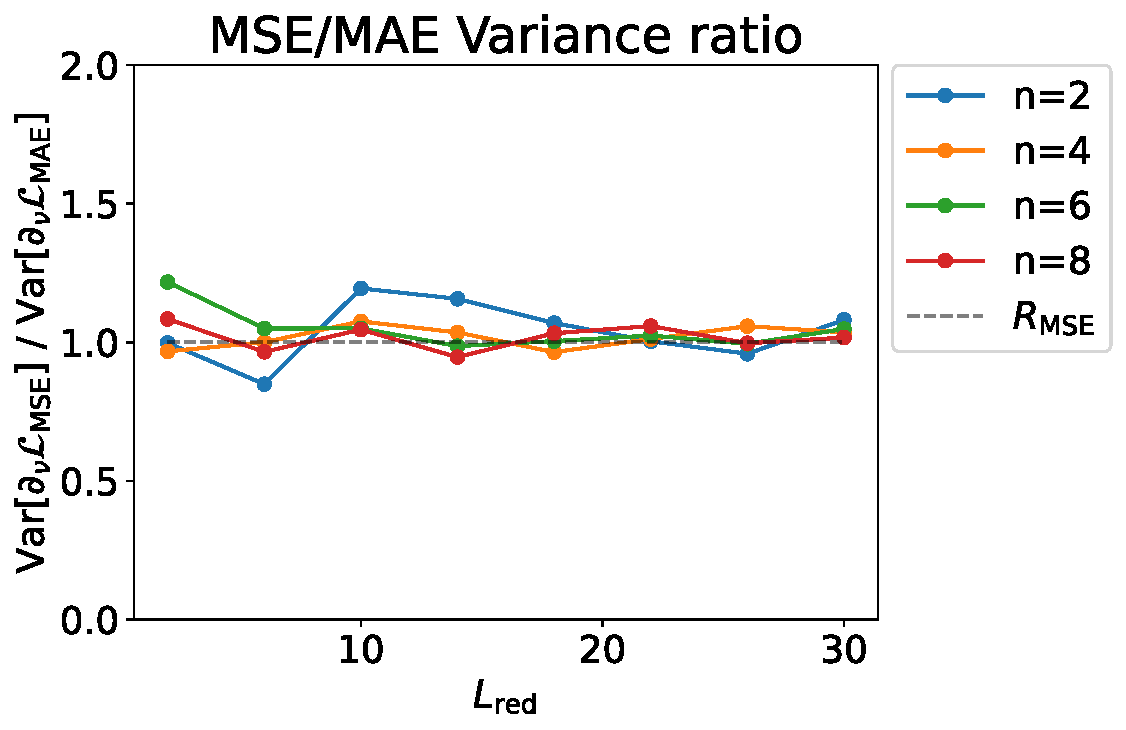
\includegraphics[width=8.5cm]{variance-mse-mae-ratio_encoding3.pdf}
    \end{minipage}
    \begin{minipage}[b]{0.5\columnwidth}
        \centering
        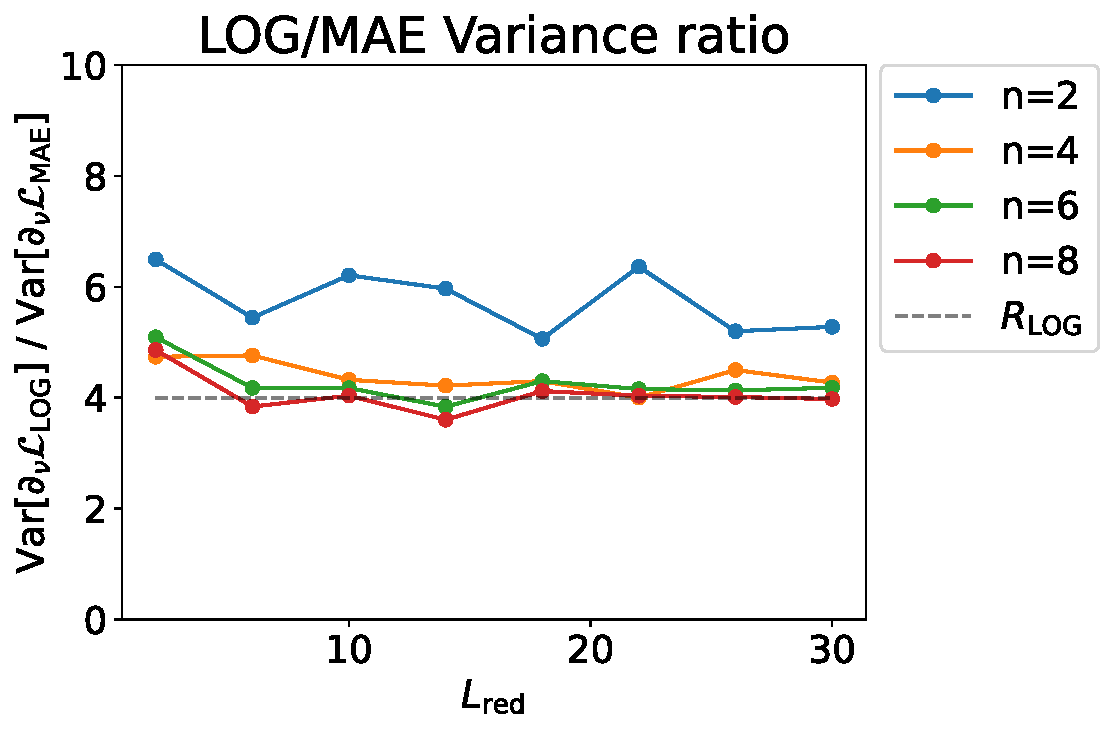
\includegraphics[width=8.5cm]{variance-log-mae-ratio_encoding3.pdf}
    \end{minipage}
    \caption{図~\ref{fig:tpa-alt-circuit}の量子回路を用いて計算したそれぞれのコスト関数の勾配の分散から、絶対誤差の勾配の分散との比を計算した。左は、二乗誤差と絶対誤差の勾配の分散の比、右は、交差エントロピー誤差と絶対誤差の勾配の分散の比をプロットしたものである。破線は、式\eqref{eq:cost-approx-var}で得られた近似比(左: $R_{\mathrm{MSE}}=1$、右: $R_{\mathrm{LOG}}=4$)を表している。}
    \label{fig:qml-var-ratio}
\end{figure}


図~\ref{fig:qml-var-ratio}の左は、二乗誤差と絶対誤差の勾配の分散の比、右は、交差エントロピー誤差と絶対誤差の勾配の分散の比である。破線は、式\eqref{eq:cost-approx-var}の近似比($1$ または $4$)を表している。
両方の数値計算の結果とも、量子ビット数 $n=2$ のときはややばらつきがあるが、各量子ビット数 $n$、学習回路の各層数 $L_{\text{red}}$ において式\eqref{eq:cost-approx-var}の近似比($1$ または $4$)に近い値をとっていることがわかる。
特に、学習回路の層数 $L_{\text{red}}$ が少なく、ユニタリ $2$--デザインを成すには不十分な場合にも、式\eqref{eq:cost-approx-var}の近似比($1$ または $4$)に近い値をとっている。量子ビット数 $n=2$ のときはばらつきがやや大きいのは、量子ビット数が少ないほど $\ell_i(\bs{\th})$ の分散が大きくなり、$\ell_i(\bs{\th}) \sim 1/2$ の近似が成り立たないためであると考えられる。

このことから、数値的にも、二乗誤差と交差エントロピー誤差のコスト関数の勾配の分散は、絶対誤差のコスト関数の勾配の分散と同程度のスケーリングであると考えられる。
したがって、バレンプラトーの解析においては、いずれかひとつについてのみ考えれば、他のコスト関数についても同様の結果が得られると推測される。


以上の議論では $O_{\rmL} = \frac{1}{n} \sum_{j=1}^{n}\dyad{0}_{j} \otimes \bbid_{\bar{j}}$ をオブザーバブルに用いたが、一般的に、Pauli 演算子の線形結合で表されるオブザーバブルを用いても、同様に $\ell_i(\bs{\th})$ の値の集中が示される。
例えば、測定するオブザーバブルを $O = c_{\bs{0}}\bbid + \sum_{\{\bs{i}\}\backslash\bs{0}} c_{\bs{i}}P_{\bs{i}}$ と表す。ただし、$P_{\bs{i}} = \bigotimes_{j=1}^n P_{i_j},\, i_j \in \{0,1,2,3\}$ であり、$P_{i_j}$ は第 $j$ 番目の量子ビットにおける Pauli 演算子、$c_{\bs{i}}$ は実数である。
このとき、$\ell_i(\bs{\th}) = \Tr[V\rho_iV O]$ の平均と分散は次のように計算される。
\begin{align}
    \E_{\calU(d)}[\ell_i(\bs{\th})]   &= c_{\bs{0}}\\
    \Var_{\calU(d)}[\ell_i(\bs{\th})] &= \frac{1}{2^n+1}\sum_{\{\bs{i}\}\backslash\bs{0}} c_{\bs{i}}^2
\end{align}
よって、$\sum_{\{\bs{i}\}\backslash\bs{0}} c_{\bs{i}}^2 \in \order{\poly(n)}$ であれば、チェビシェフの不等式から $\ell_i(\bs{\th})$ は指数関数的に $c_{\bs{0}}$ に集中することがわかる。
したがって、この節における議論は、$O_{\rmL}$ に限らず、一般的なオブザーバブルについても成り立つと考えられる。

